\documentclass[12pt]{article}
\usepackage[utf8]{inputenc}
\usepackage{amsmath}
\usepackage{graphicx}
\usepackage{amsfonts}
\usepackage{adjustbox}
\usepackage{listings}
\usepackage{color}
\usepackage{braket}
\usepackage{pgfgantt}
\usepackage{subcaption}
\usepackage{tabularx}
\usepackage{pdfpages}
\usepackage{verbatim}
\usepackage[table,xcdraw]{xcolor}

\definecolor{dkgreen}{rgb}{0,0.6,0}
\definecolor{gray}{rgb}{0.5,0.5,0.5}
\definecolor{mauve}{rgb}{0.58,0,0.82}

\graphicspath{{figures}}

\usepackage{geometry}
 \geometry{
 a4paper,
 total={170mm,257mm},
 left=25mm,
 right = 25mm,
 top=30mm,
 bottom=35mm
 }

\newcommand{\detailtexcount}[1]{%
  \immediate\write18{texcount -merge #1.tex > #1.wcdetail }%
  \verbatiminput{#1.wcdetail}%
}

\usepackage[backend=biber]{biblatex}

\addbibresource{diss.bib}

\numberwithin{equation}{section}

\nocite{*}

\lstset{frame=tb,
  language=Python,
  aboveskip=3mm,
  belowskip=3mm,
  showstringspaces=false,
  columns=flexible,
  basicstyle={\small\ttfamily},  numbers=none,
  numberstyle=\tiny\color{gray},
  keywordstyle=\color{blue},
  commentstyle=\color{dkgreen},
  stringstyle=\color{mauve},
  breaklines=true,
  breakatwhitespace=true,
  tabsize=3
}


%TC:ignore
\title{Analysis of the Quantum Advantages for Deep Hedging}

%TC:endignore

\author{Soham Deshpande\\ Supervisor: Dr. Srinandan Dasmahapatra}
\date{October 2024}

\begin{document}

\maketitle
\vspace{10cm}
A project progress report submitted for the award of MEng Computer Science
\thispagestyle{empty}

%TC:ignore
%\detailtexcount{progress}
%TC:endignore






\clearpage

\pagenumbering{roman}

%TC:ignore
\begin{abstract}
Parameterised Quantum Circuits (PQCs) have opened many doors, one 
such being the use in financial markets. In this paper, I look at the problem 
of optimally hedging a portfolio of derivatives through the use of quantum computing. 
Given a Quantum Circuit Born Machine (QCBM), we are able to generate synthetic 
data that mimics the statistical distribution of the original dataset. 
We are generating synthetic market data, here the dynamics of a 
given vanilla option's underlying is learnt. The market generator is then used to simulate the 
underlying to maturity with the intent of learning an optimal hedging strategy $\pi^*$, a 
showcase of a data-driven approach to risk hedging. Different generator architectures
will be compared to maximise the quality of the synthetic data. The findings of 
this research will contribute to the growing literature on risk management in 
quantitative finance, with applications of the market generator extending beyond 
deep hedging. 
\end{abstract}

\clearpage


\tableofcontents
%TC:endignore
\clearpage



\pagenumbering{arabic}


\section{Problem Statement}
The problem of hedging a portfolio of derivatives is an important part of 
risk management used widely in financial institutions. We can picture a perfect, 
frictionless market where transaction costs are negligible and every asset in 
the space has a price. Here we can price and hedge perfectly. Unfortunately in 
practice, we experience incomplete markets due to frictions. In recent years 
markets have experienced periods of heightened volatility, much that disobey 
traditional frameworks. This generates the need for complex, realistic market 
models that can account for these.\\ 
Traditional methods of hedging options has shown to be ineffective for equity 
markets, new information resulting in rapid changes. Much of the available 
literature models the market as a smooth, continuous stochastic process within 
a Gaussian space. Such models are sufficient for common market activity but fail 
when presented with discontinuous moves in price. In the context of Euro Stoxx 50, 
these can be reactions to geopolitical events or natural disasters; traditional
models are incapable of capturing the effects. The introduction of Jump-diffusion 
models aimed to solve this issue though face similar issues. In reaction, we have 
recently observed non-parametric models that harness neural networks and machine 
learning which aim to demonstrate high accuracy on out-of-sample forecasts.
\\
In the deep hedging framework, we are able to construct a dynamic optimal hedging 
policy by following realistic market simulations to maturity. This is a policy 
that involves 
a mapping from market states to actions. Instead of solving analytical equations 
under unrealistic market assumptions, such as Greek hedging, we can instead model
the trading decisions made as an optimisation problem, particularly suitable for 
neural networks with a rich feature set. I will be focusing on the 
accuracy of the market simulation itself; through the utilisation of quantum computing 
techniques, I wish to enhance market simulations so that a more optimal hedging strategy 
can be learnt than prior techniques. In this, an exploration into quantum circuit 
architectures will be conducted, as well as exploiting quantum machine learning 
for the simulation and policy search.

\clearpage
\section{Related Literature}
To place this research within the context of existing literature, we can split 
the project into 2 components: the market generator, and quantum parameterised circuits.
\\
The work around deep hedging has evolved, moving away from 
Greek-based hedging towards a sturdier framework using machine 
learning. Here a lot of work is being done, with many papers emphasising 
on using neural networks for optimising delta and gamma exposure
\autocite{armstrong_deep_2024,qiao_enhancing_2024}.
Buehler introduced an approach, modelling trading decisions 
as neural networks instead of relying on parameterised models
\autocite{buehler_deep_2019}. Subsequent advancements focussed on developing realistic market simulators. Wissel 
proposed a market model for path generation of options but this still 
employed risk-neutral diffusion\autocite{schweizer_arbitrage-free_2008}. Wiese then introduced 
a new dimension by using GANs to convert options into 
local volatility models with simpler no-arbitrage constraints. This focussed 
on the local stochastic nature of options
\autocite{choudhary_funvol_2023,wiese_deep_2019,wiese_multi-asset_2021}.
Some approaches suggest using actor-critic reinforcement learning algorithms to 
solve for an optimal value function, a move towards searching for a global
maximum over local risk management
\autocite{buehler_deep_2022,movahed_introducing_2024}.
\\
Recent research explores using quantum computing to 
hedge portfolios, here the authors presented a quantum reinforcement learning 
method based on policy-search and distributional actor-critic algorithms. 
They proposed using a Quantum Neural Network to approximate the value of a 
given value function by predicting the expected utility of returns using compound and orthogonal layers which were built using Hamming-weight
unitaries\autocite{kerenidis_classical_2022}. This helped overcome the barren plateau by ensuring the gradient 
variance does not vanish exponentially with qubit count. Another method models the entire return distribution, leveraging parameterised circuits to learn categorical distributions and capture variability and tail risk 
\autocite{cherrat_quantum_2023,dasgupta_loading_2022}.
\\
There is an immense amount of research being done on exploiting the benefits of 
quantum computing, recent advancements being in quantum algorithms. 
These claim to provide exponential speed-up over classical 
methods, though in reality, we see great complexity in state preparation, requiring 
$\Theta(2^n/n)$ circuit depth with n qubits or $\Theta(n)$ circuit depth with 
$\Theta(2^n)$ ancillary qubits\autocite{zhang_quantum_2022}. Here we see hybrid models such as Born machines
and Quantum generative adversarial networks boasting high generalisation ability
\autocite{ganguly_implementing_nodate,gili_2022_do,horowitz_quantum_2022}.
\\
There has also been research in harnessing back action from quantum weak 
measurements to enhance the ability of quantum machine learning algorithms. 
In quantum reservoir computing,
the ability to retain information from past inputs plays a key role in processing 
temporal series and producing future predictions
\autocite{franceschetto_harnessing_2024,fujii_quantum_2020,garcia-beni_squeezing_2024,mujal_time-series_2023}.
\\
This research aims to combine the needs of financial firms in hedging portfolios
using realistic market models by utilising QCBMs as a tool 
for simulating paths in combination with quantum neural networks for learning 
optimal policies. A comparison will be made against hedging under Black-Scholes.


\clearpage
\section{Markets and Derivatives}
The market, though inherently can be thought of as a completely random process,
where bids and asks are fulfilled, can be modelled as a stochastic process. The 
aim of this chapter is to serve as a brief introduction and set up notation for 
later chapters. \\
\subsection{Market}
Consider a market with a finite time horizon $T$ defined on the probability space 
($\Omega,\mathcal{F},P$) along with a filtration $\bold{F} = \{\mathcal{F}| 0 \leq t \leq T \}$ 
This can be thought of as an adapted (n+1) dimensional It\^{o} process 
$X(t) = (X_0(t), X_1(t),...,X_n(t))$
which has the form 
\begin{equation}
dX_0(t) = \rho(t,\omega)X_0(t)dt;\hspace{8pt}X_0(0)=1
\end{equation}and
\begin{equation}
dX_i = \mu_i(t,\omega)dt+\sigma_i(t,\omega)dB(t);\hspace{8pt}X_i(0)=x_i 
\end{equation}
where $X_i(t)$ as the price of asset $i$ at a given time $t$.
\\
We can define a portfolio in the market as 
\begin{equation}
\theta(t,\omega) = (\theta_0(t,\omega),\theta_1(t,\omega),...,\theta_n(t,\omega))
\end{equation}
where the components $\theta_n(t,\omega)$ represents the number of units of a given 
asset held at time $t$.\\
Following from that, we can define the value of a given portfolio to be 
\begin{equation}
  V(t,\omega) = V^{\theta}(t,\omega) = \sum_{i=0}^n \theta_i(t)X_i(t)
\end{equation}
Lastly, it is important to state that the portfolio is self-financing, any 
trading strategy $\alpha$ requires no extra cost beyond the initial capital
\begin{equation}
  V(t) = V(0) + \int_0^t\theta(s)\cdot dX(t)
\end{equation}
We can also make the following assumptions about the market:
\begin{itemize}
  \item The market is liquid, allowing the trade to execute instantaneously
  \item There is no bid-ask spread, the price to buy and sell is the same 
  \item Trading actions taken have no impact on the price of the asset traded 
\end{itemize}


\subsection{Derivatives}
A derivative refers to any financial instrument whose value is derived from an 
underlying security, the most fundamental being futures and options.
\subsubsection{Futures}
A futures contract is a contract that gives the right and obligation to buy a 
given asset $i$ a specified time $T$ at price $K$. 
\subsubsection{Options}
The two types of options going to be explored are Puts and Calls; a Call option 
gives the owner the right but not the obligation to buy a given asset $i$ at 
a specified price $K$ at time $T$. Similar to the Call, a Put option gives the 
owner the right but not the obligation to sell a given asset $i$ at a price $K$ 
at time $T$. If the owner can exercise the option any time up to $T$, we call 
this an American option. For the purposes of this research, I will only be 
dealing with vanilla European options.\\ 
It is important to define the payoffs for both options: 
\begin{equation}
C_T = max(0,S_T-K)
\end{equation}
\begin{equation}
P_T = max(0,K-S_T)
\end{equation}



\subsection{Euro Stoxx 50}
In this research I will be focussing on a single asset, the Euro Stoxx 50 Index
(SX5E) and relevant derivatives. This is a stock index of 50 stocks in the Eurozone. 
This index captures around 60\% of the free-float market capitalisation of the 
Euro Stoxx Total Market Index which covers about 95\% of the free-float market 
in the Eurozone\autocite{a2021_euro}. Rationale behind choosing this index is the availability of data,
options traded with SX5E as the underlying and the liquidity of the index.
\\
Derivatives that are held in the portfolio to be hedged will include those that 
have SX5E as the underlying, examples are weekly, monthly, and quarterly
expiration options. These are European-style so can only be exercised upon 
maturity. Data can be found on Bloomberg\autocite{bloomberg_2023_bloomberg} and Refinitiv
\autocite{lseg}.
\begin{figure}[h]
    \centering
    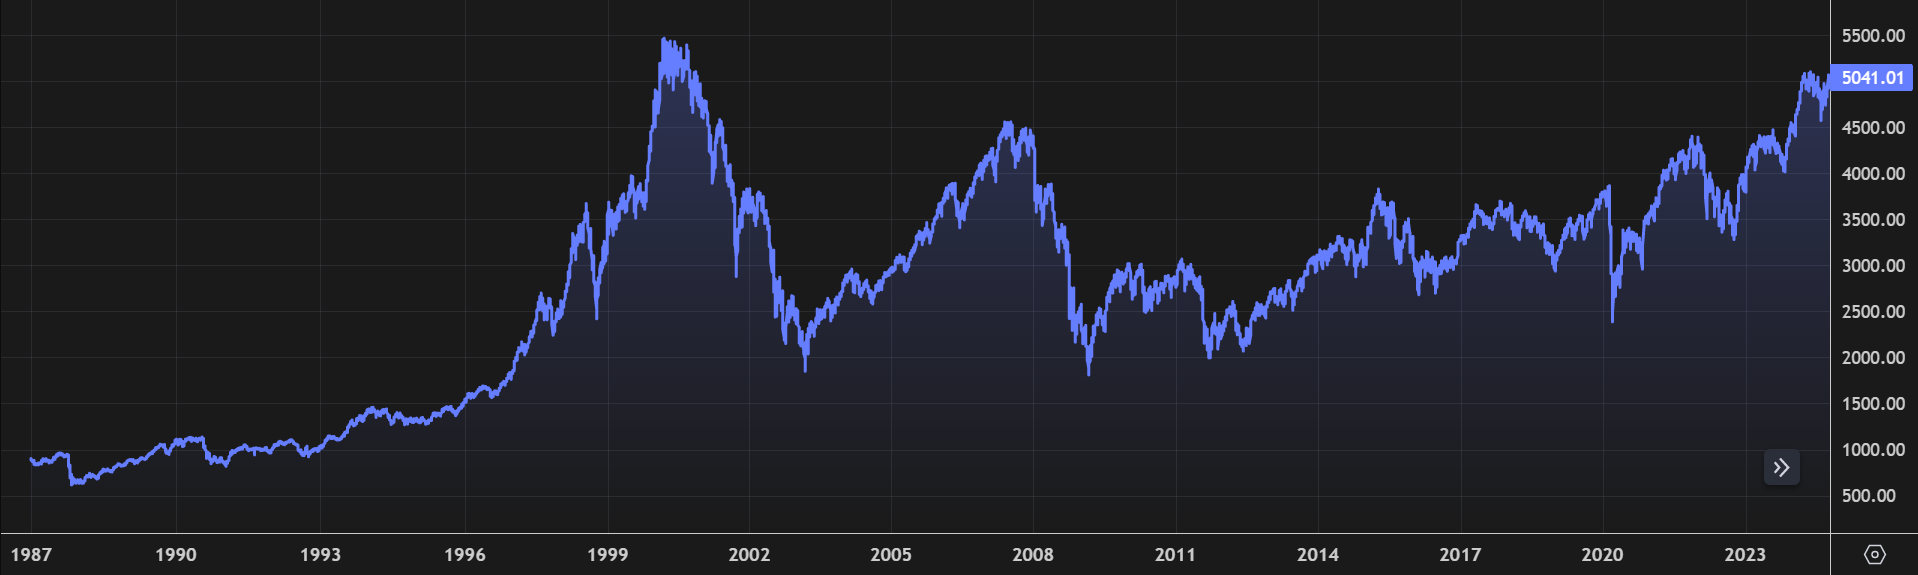
\includegraphics[scale=0.35]{sx5e.png}
    \caption{Euro Stoxx 50 price chart}
\end{figure}

\clearpage
\section{Deep Hedging}

Hedging can be thought of as a stochastic control problem where we have 3 actors, 
a market state, randomness from market returns and a hedging strategy. By making 
observations on the market state we are required to make adjustments to one's
hedging policy. 
\\
We can formally define hedging as :
$$\min_{\theta \in \Theta} \rho (H^\theta - P)$$
where $\Theta$ is the set of admissible hedging strategies, $P$ is the uncertain 
payoff of derivative at final time, $H^\theta$ is the uncertain payoff of hedging 
portfolio if strategy $\theta$ is used at final time, and $\rho$ is a risk measure.
\\
It can be assumed that the hedging instrument used, SX5E in this case, can be 
traded with sufficient liquidity and that the trading of the asset does not 
influence the price. Given these conditions, we can formulate the problem of deep 
hedging to be a reinforcement learning one. 
\\
We can set up two sets of rewards, R, positive from the cash flows from the 
portfolio of hedging instruments and derivatives. The second is C, the negative 
reward associated with transaction costs. For simplicity, we can assume that the 
cost is proportional to the cost of the hedging instrument. By taking a set of 
actions at each time step, t, we can formulate a trading strategy which gives an 
expected return of
$T^\pi_t = (R^\pi_{t+1} - C^\pi_{t+1} )+ ... +(R^\pi_T - C^\pi_T)$.
The goal of the reinforcement algorithm would be to maximise the expected return. 
However, to create a strategy that does not incur too much risk, it is important 
to include metrics such as Value at Risk (VaR) and Conditional Value at Risk(CVAR)
where
\begin{equation}
\text{VaR}_{\alpha}(X) = \inf \{x \in \mathbb{R} : P(X \leq x) \geq \alpha \}
\end{equation}
and likewise,
\begin{equation}
\text{CVaR}_{\alpha}(X) = \frac{1}{1 - \alpha} \int_{-\infty}^{\text{VaR}_{\alpha}(X)} x \cdot\, p(x) \, dx
\end{equation}
These aim to minimise the tail-risk involved in a given trading strategy hence 
creating a more robust strategy and conforming to regulations such as Basel III
\cite{saissihassani_2021_the}.
\\
One of the main problems is the scarcity of data, calibration of such models 
requires huge amounts of realistic market data for the underlying. Hence this
requires a market generator. Traditionally a GBM with Monte Carlo simulations 
would be used but this paper goes beyond, using quantum computing to combat the 
aforementioned issues. 
\\
The design of the neural network responsible would involve an input layer which
takes the market state such as the underlying, and options features such as the 
strike price and maturity.\\
The loss function will have
type: $\text{Loss }=\lambda_1\cdot\mathcal{L}_R + \lambda_2 \cdot \mathcal{L}_{CVaR}$
where $\lambda_i$ is the weighting of the two losses, $\mathcal{L}_R$ 
is the replication loss from simulating the options to maturity given a generator. 
We can define it as $\mathcal{L}_R(X^\alpha_T-g(S_t))$ where $X^\alpha_T$ is the 
portfolio at maturity and $g(S_t)$ is the option pay-off.
\\
This takes a global approach towards finding an optimal policy instead of 
managing a local criterion as suggested by \cite{fecamp_deep_2021}.


\clearpage 
\section{Parameterised Circuits} 
\subsection{Born Rule}
An essential part of quantum computing involves the existence of the Born
Rule. Born's measurement rule states that:
\begin{equation}
p(x) = |\langle x|\psi(\theta)\rangle|^2
\end{equation} where 
\begin{equation}
|\psi(\theta)\rangle = U(\theta)|0\rangle^{\otimes n}
\end{equation}
The state $|\psi(\theta)\rangle$ is generated by evolving state $|0\rangle$
according to a Hamiltonian $H$ that is constructed from gates. Once combined, the 
gates form a parameterised quantum circuit which is parameterised by using the 
variables governing each gate, $\theta$. By tuning the values of $\theta_i$ one 
can allow for an evolution to any state that will serve as a solution to a given 
problem. \\ 
By taking the distribution associated to the state, $|\psi(\theta)\rangle$ we can 
treat the PQC as a generative model, upon measurement will 
generate samples of a target distribution $\chi$. This model is parameterised 
by $\theta$, which defines a quantum circuit $U(\theta)$ made up of a set of quantum 
gates.
By measuring the circuit, we can obtain samples. Producing samples that emulate 
the target distribution involves minimising the parameters of the circuit $U(\theta)$, 
a process once convergence is reached, will generate accurate samples 
\cite{liu_differentiable_2018}.

\subsection{State Preparation}
We require state preparation to transfer the classical data onto the 
Hilbert space. This involves a function $\phi$ that maps the input vector to 
an output label. There are many encoding schemes, each of which aim to offer 
high information density and low error rates; main methods include: basis, amplitude, angle encoding, and QRAM. 
\\
Without the use of ancillary qubits, we can expect an exponential circuit depth
to prepare an arbitrary quantum state. Using them we can reduce the depth to be 
sub-exponential scaling, with recent advancements reaching $\Theta(n)$ given $O(n^2)$
ancillary qubits
\cite{shaib_efficient_2023,zhang_quantum_2022}.


\subsubsection{Amplitude Encoding}
Amplitude encoding consists of the following transformation:\\
\begin{equation}
S_X \ket{0} = \frac{1}{||x||}\sum^{2n}_{i=1}{x_i\ket{i}}
\end{equation}
where each $x_i$ is a feature of the data point x, and $\ket{i}$ is the basis 
of the n-qubit
space. This does boast the advantage of being able to store $2^n$ features using 
only n qubits but does create a resultant circuit with depth $O(2^n)$.

\subsubsection{Angle Encoding}
The transformation used is:
\begin{equation}
S_x\ket{0} = \otimes^n_{i=1} cos(x_i)\ket{0} + sin(x_i)\ket{1}
\end{equation}
It can be constructed using a single rotation with angle $x_i$ which is 
normalised to be within $[-\pi,\pi]$. This allows us to store $n$ features with 
$n$ qubits.
\\
A possible encoding method is dense angle encoding which allows us to encode $2n$ 
features in n qubits but hasn't been chosen in this project for simplicity.


\subsection{Measurements}
In quantum mechanics, we can define measurement to be any process that probes a 
given quantum system to obtain information, we may also refer to this process as 
a measurement in the computational basis when focussing on quantum information 
science. Let's consider a quantum state 
$|\psi \rangle = \alpha_0|0\rangle+\alpha_1|1\rangle$ which gives us $|0\rangle$
with probability $|\alpha_0|^2$ and $|1\rangle$ with probability $|\alpha_1|^2$. 
If measured in the standard basis we would expect the outcome to be $|k\rangle$
with a given probability. This outcome would result in the output 
state of the measurement gate to also be $|k\rangle$, resulting in the original 
state $|\psi\rangle$ to be irreversibly lost. We can refer to this as a collapse of state. 


\subsection{Quantum Circuit Born Machine}
Given a dataset $D = \{x_1, x_2.. x_n\}$ consisting of n samples and obeys a 
given distribution $\chi_d$, we would like the QCBM to learn the distribution 
and generate synthetic data points that are of the distribution $\chi_s$ such that
$\chi_s$ approximates $\chi_d$.
The QCBM is a subclass of parameterised quantum circuits, 
here the quantum circuit contains parameters which are updated during a training 
process. The QCBM takes the product state $\ket{0}$ as an input, and through an 
evolution, transforms into a final state $\ket{\phi_0}$ by a sequence of unitary 
gates. This can then be measured to obtain a sample of bits 
$x \sim p_\theta (x_s)=|\bra{x}\ket{\phi_\theta}|^2$ . By training the model we 
are aiming to let $p_\theta$ approach $\chi_d$. 
\\
The ansatz for this quantum circuit consists of 7 layers
of 1-qubit gates with entangling layers in between them. These are 
entangled using the CNOT gates as found in the appendix. The number of wires 
needed depends on the precision required for the generated data. The estimated
precision is 12-bit, so the samples are able to take $2^{12}$ different values in 
the range of $ (v_{min} - \epsilon, v_{max} + \epsilon )$, where $\epsilon > 0 $
allows data to be generated that lie outside the range $(v_{min},v_{max})$ of the 
original data.
\\
The QCBM takes a $n \times m$ matrix of parameters in the range $(-\pi, \pi)$ as 
input, in the form of a dictionary. Each angle takes one of $2^k$ discrete values, 
where $k$ is a model parameter. The resulting space therefore spans to: 
$(2^m)^{n\cdot m}$.
\clearpage
\subsubsection{Testing}
Many methods were explored to generate time-series data from the QCBM as well as 
testing parameters of the model. The first idea explored involved learning the 
distribution of the delta value of an American option.
\begin{figure}[h]
    \centering
    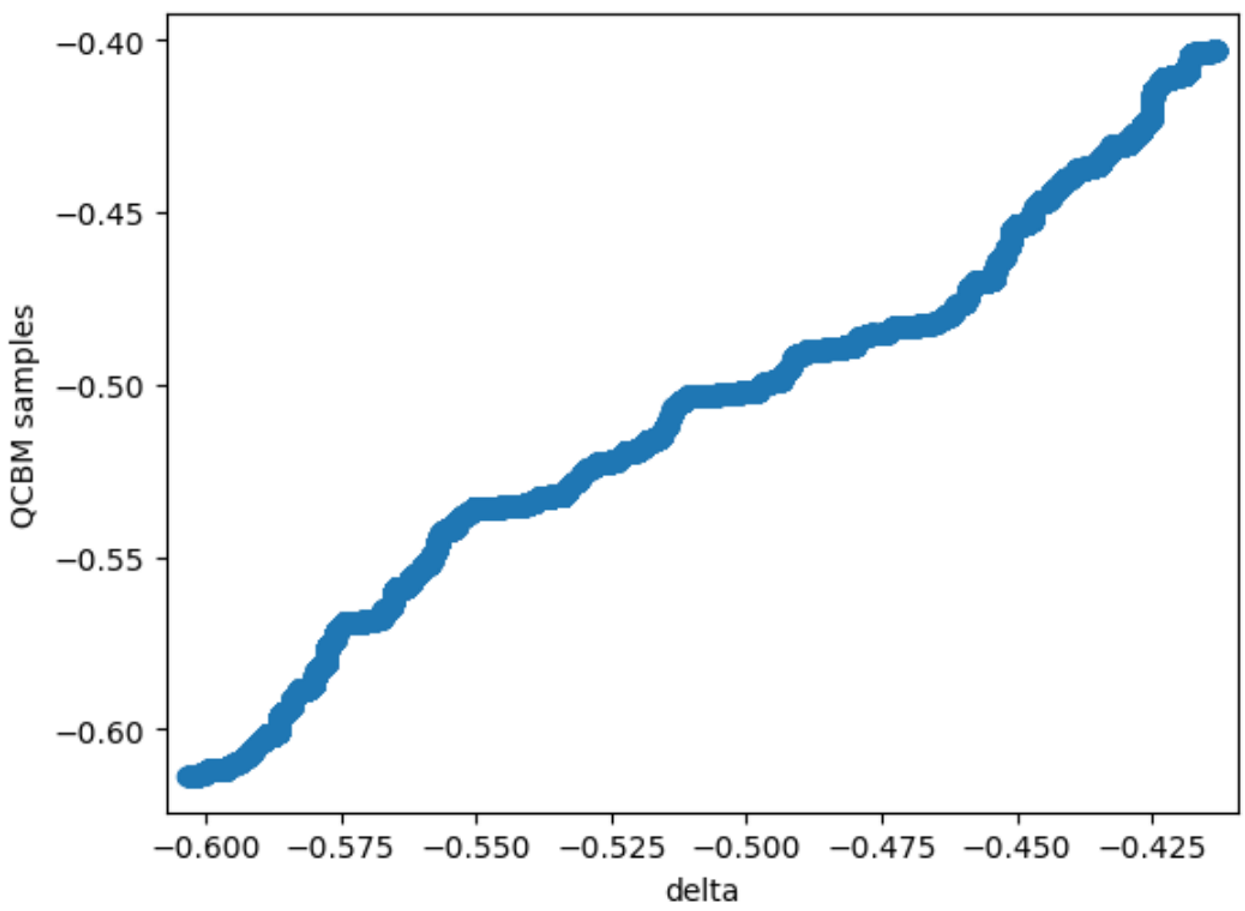
\includegraphics[scale=0.24]{QCBM-delta.png}
    \caption{Quantile plot for American option delta}
\end{figure}
\\
Given the delta of an option throughout a day, the QCBM demonstrated high
generalisation power as shown by the diagonal nature of the plot. A genetic 
algorithm was employed to learn the set of parameters $\theta$.
The circuit also provided promising returns when learning the vega of the same 
option. 
\begin{figure}[h]
    \centering
    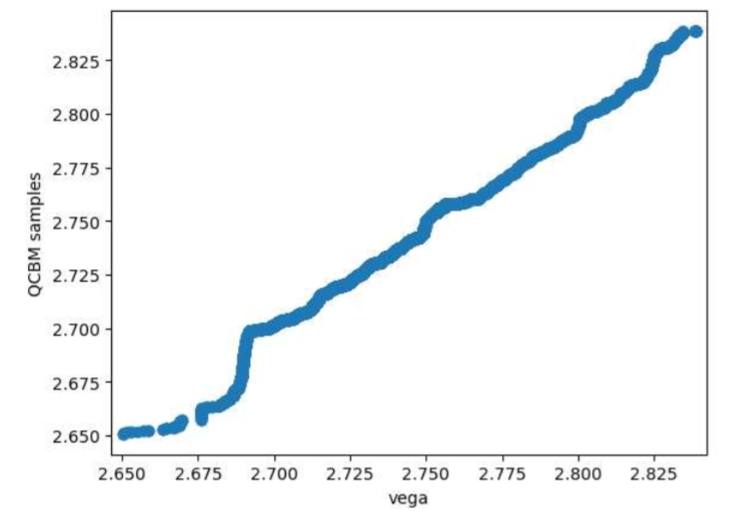
\includegraphics[scale=0.75]{QCBM-vega.png}
    \caption{Quantile plot for American option vega}
\end{figure}
\\
It was also important to verify the generalisation by learning the strike price,
which was a constant for the option. We can observe the two histograms of the 
samples generated from measurement.
\begin{figure}[h]
    \centering
    \begin{subfigure}[b]{0.45\textwidth}
        \centering
        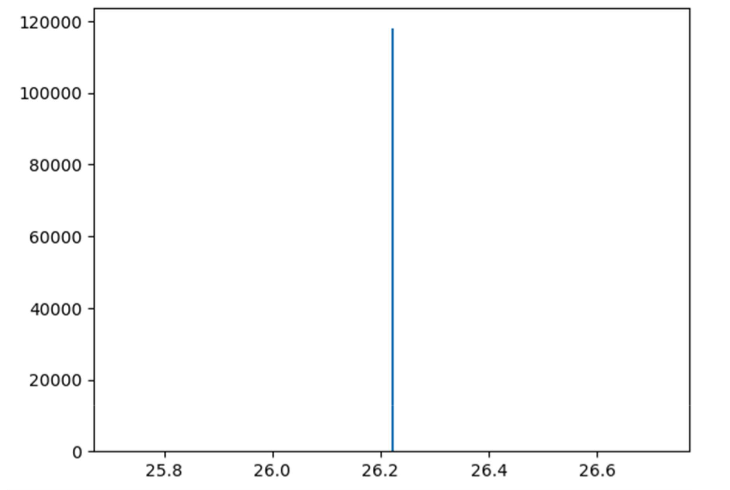
\includegraphics[scale=0.6]{QCBM-strike1.png}
        \caption{Histogram of training data}
    \end{subfigure}
    \hfill
    \begin{subfigure}[b]{0.45\textwidth}
        \centering
        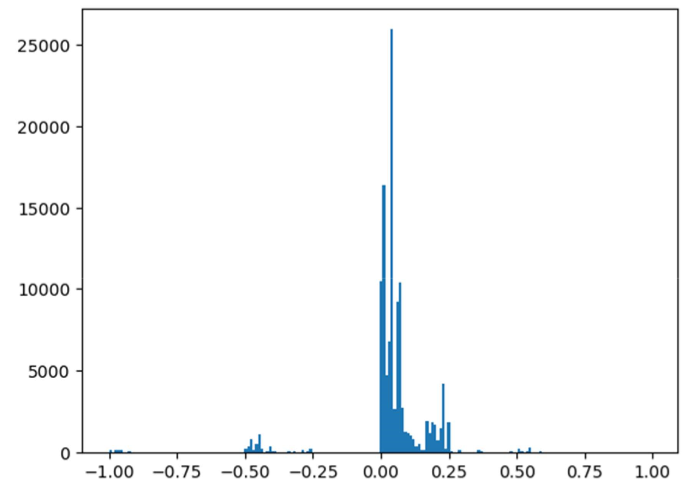
\includegraphics[scale=0.6]{QCBM-strike2.png}
        \caption{Histogram of samples observed}
    \end{subfigure}
    \caption{Comparison of training data and observed samples}
    \label{fig:comparison}
\end{figure}
\subsection{Quantum Feature Maps}
Another method for encoding time within quantum circuits was the use of
quantum feature maps. We can define this to be $\phi : X \rightarrow F$ where $F$
is a Hilbert space. This map transforms $x \rightarrow |\phi(x)\rangle$ by  $U_\phi(x)$\autocite{paine_quantum_2023,steinbrecher_quantile_2008,vlasic_quantum_2024} .
\\ 
Here we have two parts, the latent variable and time encoding. The latent variable 
is a random, uniform $z \in [0,1] $. This is encoded through the use of $R_x(\phi)$ where 
\begin{equation}
R_x(\phi) = 
\begin{bmatrix}
\cos(\phi/2) & -i\sin(\phi/2) \\
-i\sin(\phi/2) & \cos(\phi/2)
\end{bmatrix}
\end{equation}
Time in encoded through the use of $R_y(\phi')$ where 
\begin{equation}
R_y(\phi') = 
\begin{bmatrix}
\cos(\phi'/2) & -\sin(\phi'/2) \\
\sin(\phi'/2) & \cos(\phi'/2)
\end{bmatrix}
\end{equation}
It goes that by learning the quantile function of a SDE, we can evaluate it at 
random uniform $z$'s as $t$ progresses to give a time-series that obeys the 
SDE. To do so we require a circuit that maps $z$ to a sample $G(z) = Q(z)$. \\ 
I have taken the example of the Ornstein-Uhlenbeck process to provide a proof of 
concept. We can define OU to be: 
\begin{equation}
  dX_t = \theta (\mu - X_t) \, dt + \sigma \, dW_t 
\end{equation}
where $\theta$ is the mean reversion, $\mu$ is the long-term mean, $\sigma$ is the 
volatility and $W_t$ is the Weiner process. 
\\
By way of Fokker-Plank, we can get the following for the quantile function:
\begin{equation}
  \frac{\partial Q(z,t)}{\partial t} = f(Q,t) - \frac{1}{2}\frac{\partial g^2(Q,t)}
{\partial Q} + \frac{g^2(Q,t)}{2}(\frac{\partial Q}{\partial z})^{-2}
  \frac{\partial ^2Q}{\partial z^2}
\end{equation}
where $f(Q,t)$ is the drift term and $g(Q,t)$ is the diffusion term.
Training the quantum circuit requires a dataset generated from the probability 
distribution for the market, here represented by the OU process. We have to assume
the underlying SDE generates data similar to the observed data points. The loss 
function would included two parts: $\mathcal{L} = \mathcal{L}_{Data} + 
\mathcal{L}_{SDE}$. This ensures the distribution learnt conforms to a given 
known process whilst replicating dynamics observed in real life. This technique 
shines in a context where data is sparse. In this paper, I will aim to test the 
market generator using the OU process as well as a Merton Jump Diffusion model.
\begin{figure}[ht!]
    \centering
    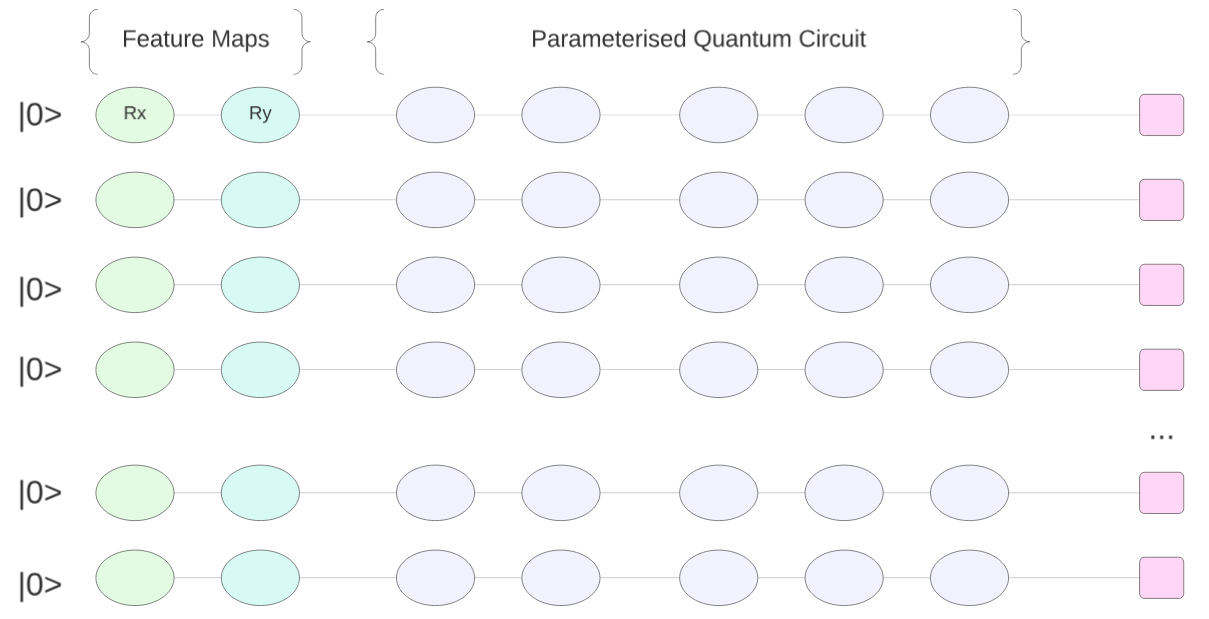
\includegraphics[scale=0.45]{qfc.png}
    \caption{PQC for representing a time-dependent quantile function }
\end{figure}

\begin{figure}[ht!]
    \centering
    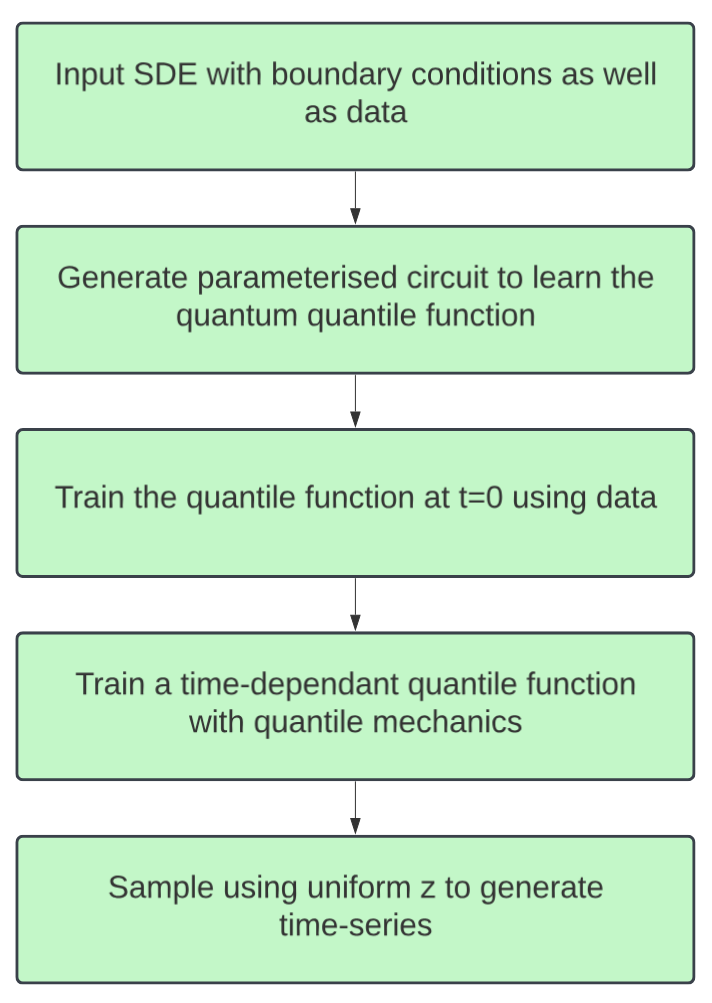
\includegraphics[scale=0.35]{qf.png}
    \caption{Quantile Function process for time-series with data}
\end{figure}
\subsubsection{Merton Jump Diffusion Model}
The MJD model is an exponential L\'{e}vy model of the form 
\begin{equation}
  S_t = S_0e^{\mathcal{L}_t}
\end{equation}
where the stock price process is modelled as an exponential of a L\'{e}vy process. 
We can also define $\mathcal{L}_t$ to be 
\begin{equation}
  \mathcal{L}_t = (\alpha - \frac{\sigma^2}{2}-\lambda k)t + \sigma B_t + 
  \sum^{N_t}_{i=1}Y_i
\end{equation}
where the first term is a Brownian motion with drift and the latter is a 
compound Poisson jump process. 
\clearpage
\subsubsection{Testing}
Using this, I was able to run some preliminary tests.
\begin{figure}[h]
    \centering
    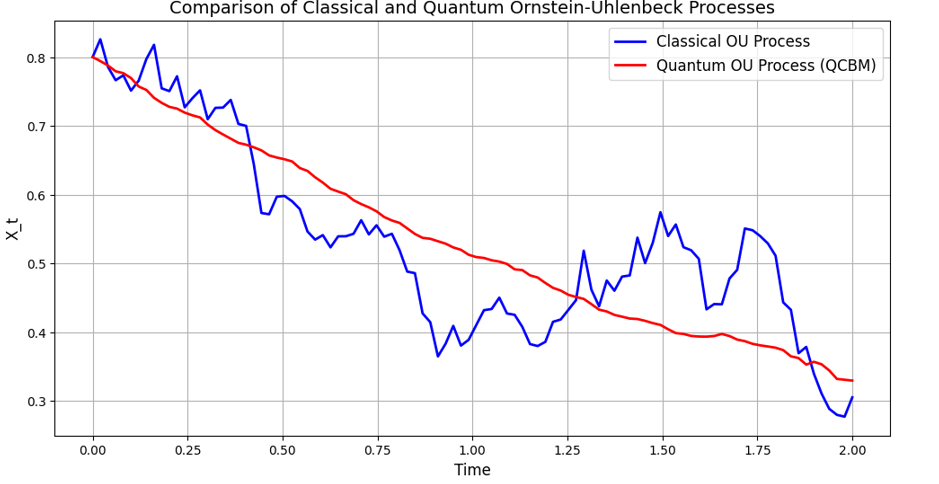
\includegraphics[scale=0.7]{Quantile1.png}
    \caption{Sampling learnt QF for the OU process}
\end{figure}
\begin{figure}[h]
    \centering
    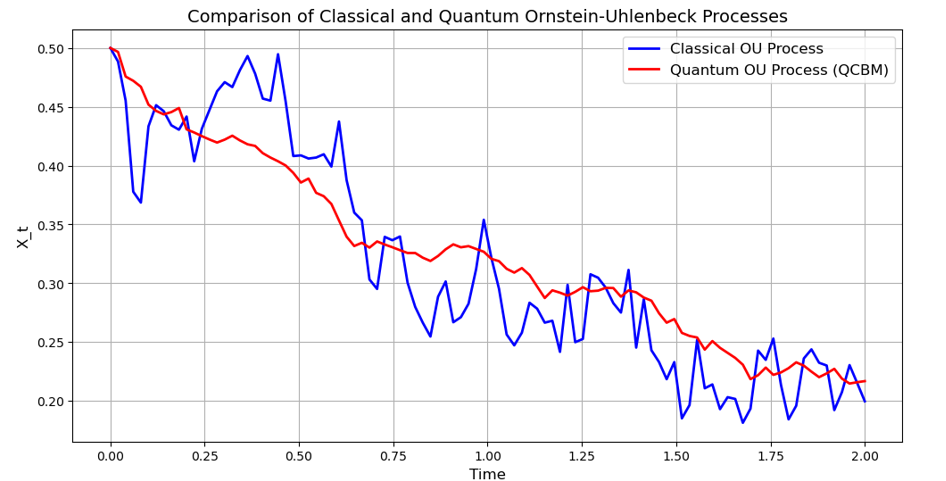
\includegraphics[scale=0.7]{Quantile2.png}
    \caption{Sampling learnt QF with higher circuit depth}
\end{figure}

\subsubsection{Barren Plateau}
A point of concern when searching for the optimal set of $\theta s$ is the large search space, here we may observe issues such as barren plateau(BP). BP 
insists that the gradient of the parameters of a given PQC will vanish exponentially 
w.r.t the search space. A formal proof can be found in\autocite{ragone_2024_a}. 
\\ 
I will aim to explore using gradient-based methods as well as alternatives such 
as genetic algorithms. 
\subsection{Design}
Below is the rough proposed high-level design with a few components. The market 
simulation of the underlying will feed into the deep hedger. The trained model 
will then be compared to a simple Greeks-based hedger on a GBM underlying.
\begin{figure}[h!]
    \centering
    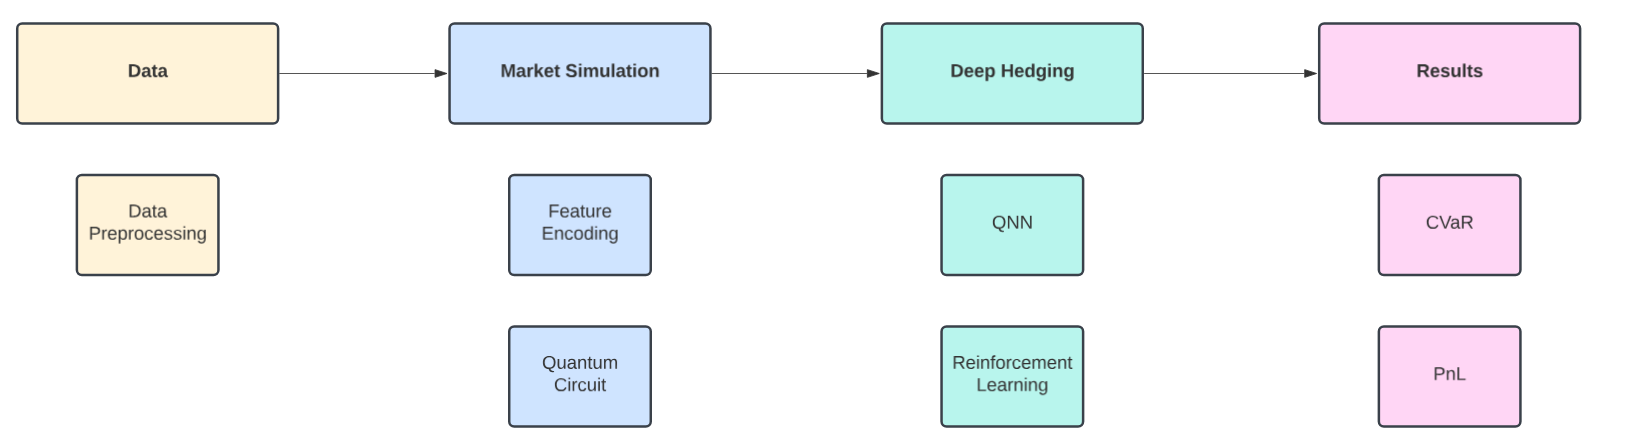
\includegraphics[width=\textwidth]{pipeline.png}
    \caption{Proposed high-level design}
\end{figure}

\clearpage 
\section{Planning}
Since this project is a solo research project, there isn't a focus on team 
management, however, increases the work required making 
time management crucial. The greatest risk identified in this project is the 
lack of convergence on a final solution as this is an emerging field with research 
being published constantly. To avoid this, a Gantt chart has been designed to 
motivate progress; this can be seen in the following figure.
\begin{figure}[htp]
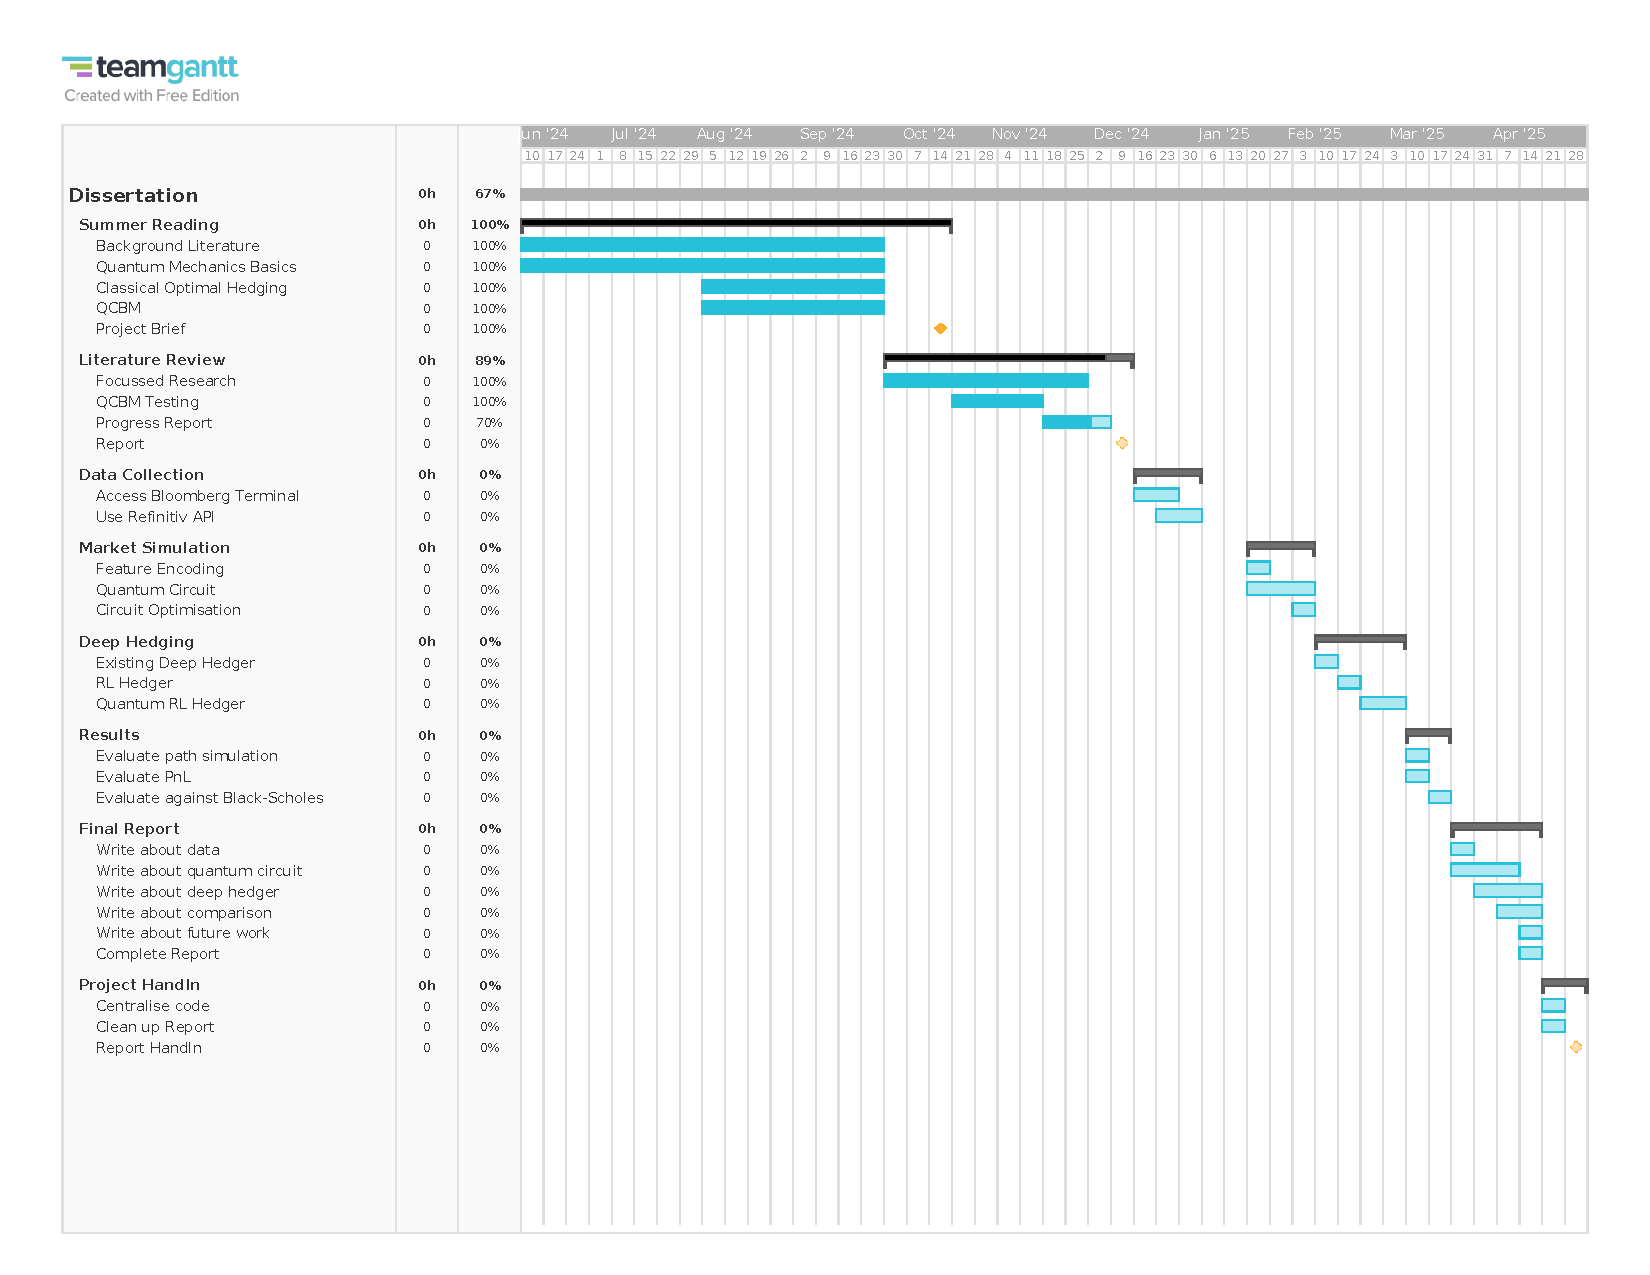
\includegraphics[page=1,width=\textwidth,scale=1.4]{GanttChart.pdf}
\end{figure}

\subsection{Agile}
Though not a team project, we can utilise some basic concepts. We can refer to 
the supervisor as a product owner. Every week progress must be shared, including 
any setbacks that may have occurred. The client can be any banks I have the 
pleasure of talking to. They can give criticism on techniques used, assumptions 
made and usefulness. I have also tried to split the project into 4 main sprints,
Data Collection, Market Simulation, Deep Hedging, and Results. They range from 
2-4 weeks dependent on the difficulty of the task at hand. The Kanban framework 
will be used for each sprint to identify and monitor tasks that need to be done. 
An example for Sprint 1 can be found in the appendix. A requirements table can 
also be found.


\subsection{Risk Assessment}
A risk assessment, though pedestrian, is included in the appendix to be holistic.\\
\clearpage


\printbibliography

\clearpage
\section{Appendix}
\subsection{QCBM Architecture}

\begin{figure}[h]
    \centering
    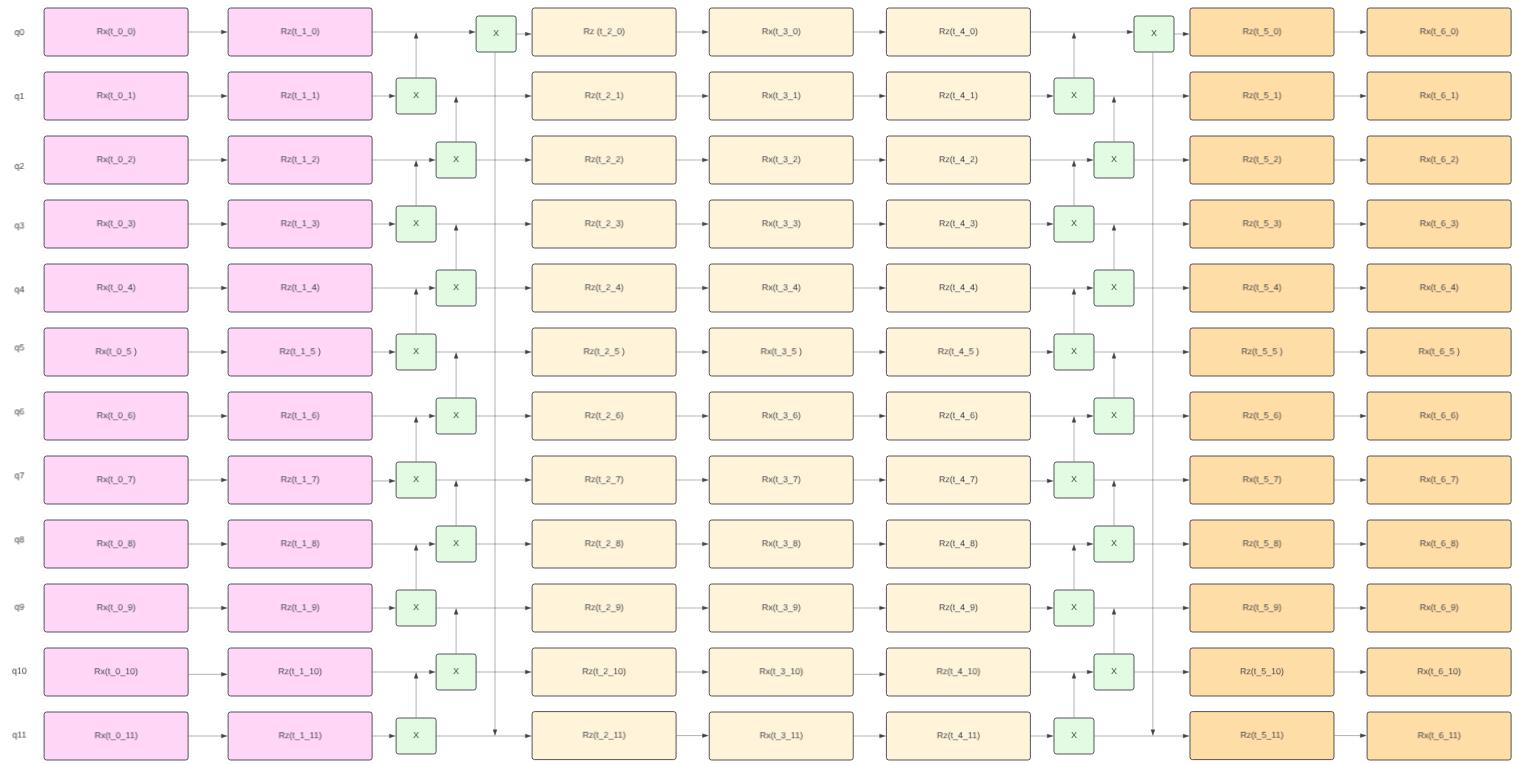
\includegraphics[scale=0.3, angle=270, width=\textwidth-209]{qcbm1.png}
    \caption{QCBM architecture}
\end{figure}
\clearpage
\subsection{Kanban}
\begin{figure}[h]
    \centering
    \includegraphics[scale=0.75]{Kanban.png}
    \caption{Example Kanban board for Sprint 1}
\end{figure}
\clearpage
\subsection{Risk Assessment}
\begin{figure}[h]
    \centering
    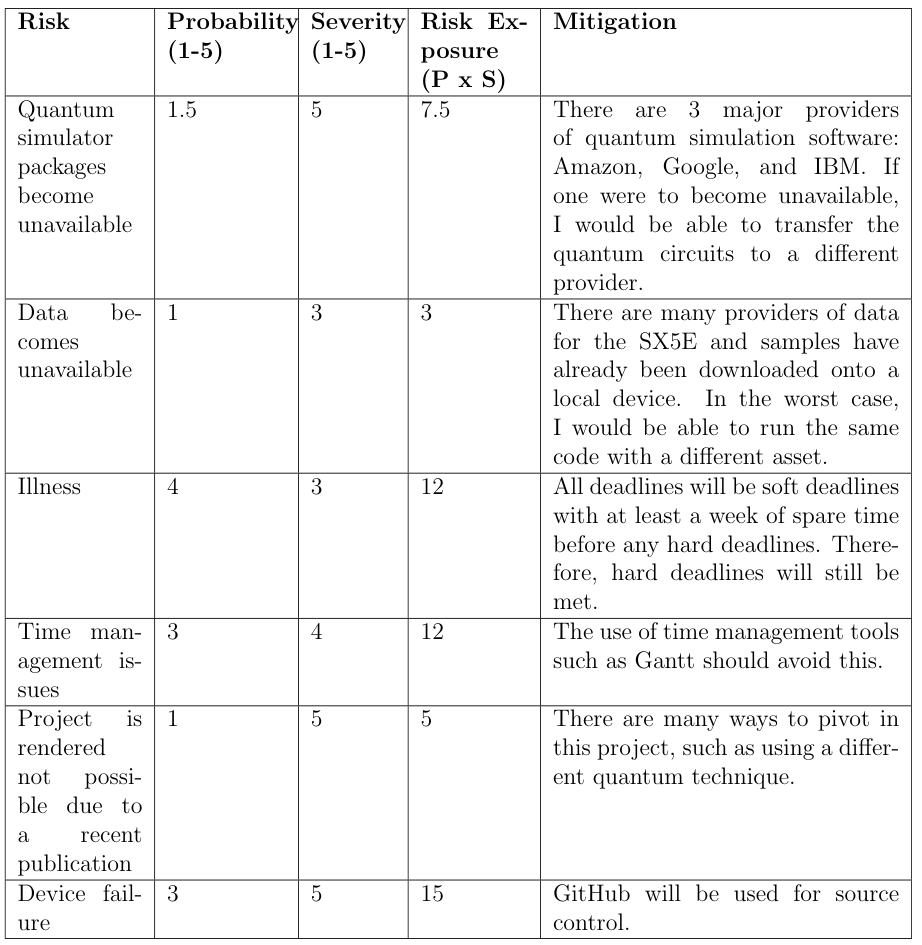
\includegraphics[scale=1]{RiskAssess.png}
\end{figure}


\clearpage
\subsection{Requirements}
\begin{figure}[h]
    \centering
    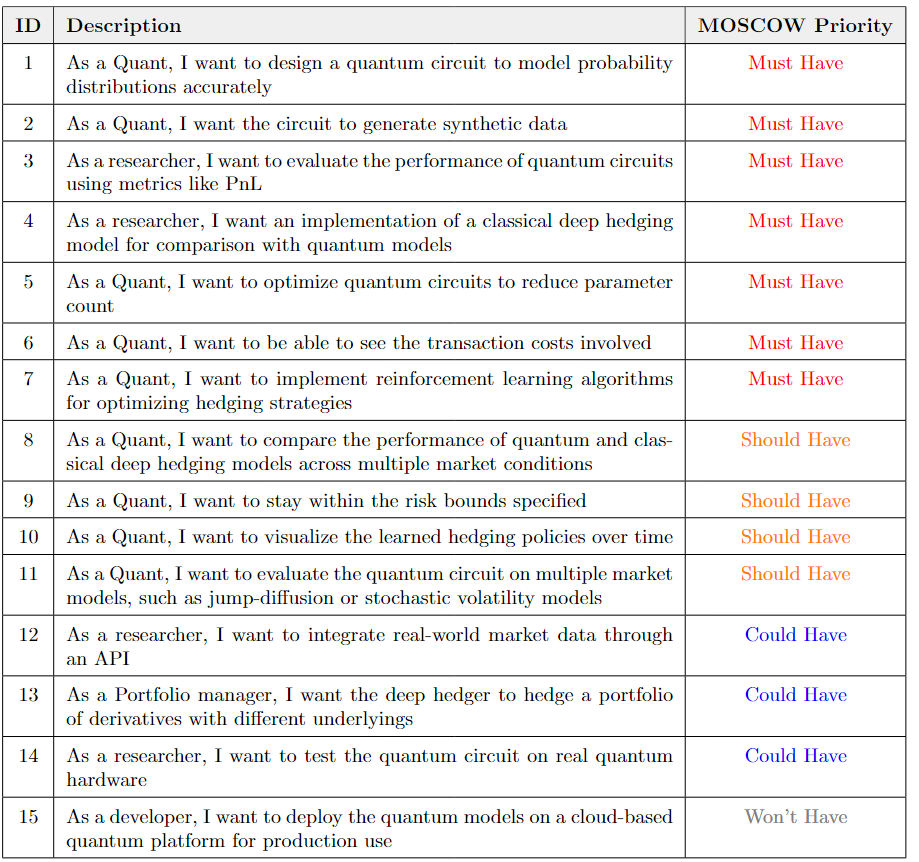
\includegraphics[scale=1.1, width=\textwidth]{requirements.png}
\end{figure}



\end{document}

